\documentclass[a4page, 14pt]{extarticle}
\usepackage{graphicx} % Required for inserting images
\usepackage{multicol}
\usepackage{caption}
\graphicspath{ {./images/} }
\setlength{\belowcaptionskip}{12pt plus 3pt minus 2pt}

\title{Rapport de première soutenance du projet Zelion}
\author{QALM\footnote{Quentin Bullier (Chef de Projet), Adrien Fonck, Louis Martin, Marcus Poirot}, entreprise Pixelicious}
\date{March 2024}

\begin{document}

\maketitle

\begin{center}
        
\includegraphics[width=8cm]{logo}
\end{center}
\captionof{figure}{Logo de l'enterprise Pixelicious}

\newpage
\renewcommand{\contentsname}{Table des matières}
\tableofcontents
\newpage

\section{Introduction}
    {Ce rapport a pour rôle pour récapituler les avancements de l'équipe QALM au moment de la premiere soutenance.}
    
\section{Objet de l'Étude (inchangé)}
    {Afin de faciliter la compréhension de ce rapport, vous trouverez ici une copie de l'Objet de l'Étude de notre jeu, déjà présent dans notre cahier des charges.}

\subsection{État de l'Art}
    {Notre jeu appartient au genre action-aventure.

    Cela signifie que le joueur explore un monde où il découvre son histoire, ses secrets et affronte toutes sortes de monstres.

    Il existe de nombreuses façons différentes de permettre à un joueur d'explorer un monde à travers son écran.}

\section{Répartition des Tâches}
    {La répartition des tâches est restée la même depuis le début. Nous avons mis en place un système de responsabilité afin de coordonner les différentes facettes du projet.\\
    Le responsable est donc plus actif sur la tâche qui lui a été assignée, cependant nous pensons que la cohésion de notre équipe fera de Zelion un bon jeu. Ainsi, tout le monde est libre de donner des critiques constructives ou des idées aux autres responsables, ainsi que de les épauler dans la programmation des différentes fonctionnalités.\\}
    \begin{center}
        \begin{tabular}{|l|c|c|c|c|}
            \hline
             & Adrien & Quentin & Louis & Marcus \\
            \hline
            Noyau du gameplay & R & S & & \\
            Interface utilisateur & R & & &\\
            IA - Ennemis & S & & R & \\
            Graphisme & & & & R\\
            Sound design & & & & R\\
            Écriture & & R & & \\
            Level design & & R & & S \\
            Multijoueur & & S & R & \\
            Equilibrage & R & R& R & R \\
            \hline
        \end{tabular}
    \captionof{table}{Répartition des tâches (R : responsable, S : suppléant )}
\end{center}
\section{Avancement}
    {Dans le tableau si dessous, vous pouvez voir nos avancements lors de la première soutenance comparé avec ce que nous avions prévu de faire.}
    \begin{center}
        \begin{tabular}{|l|c|c|}
            \hline
             & Avancement & Prévisions initiales\\
            \hline
            Noyau du gameplay & 80\% & 90\% \\
            Interface utilisateur & 30\% & 40\% \\
            IA - Ennemis & 10\% & 20\% \\
            Graphisme & 40\% & 40\% \\
            Sound design & 0\% & 0\% \\
            Écriture & 80\% & 80\% \\
            Level design & 20\% & 20\% \\
            Multijoueur & 0\% & 0\% \\
            Équilibrage & 0\% & 0\% \\
            \hline
        \end{tabular}
    \captionof{table}{Avancement des taches contre prévisions}
    \end{center}

\section{Ressenti Individuel}
    \subsection{Quentin}
        \subsubsection{Travaux Réalisés}{
    J'ai contribué à construire les bases du jeu, notamment les mouvements du personnage, les attaques du personnage (épée, arc tirant des flèches et pose d'une bombe infligeant des dégâts de zone), le rendu du jeu (y compris l'utilisation de la lumière), la structure du projet, le site web, ainsi que l'écriture et l'implémentation basique des animations. Je vais maintenant décrire chaque partie, et dans la prochaine partie, je partagerai mes impressions sur chacune d'entre elles.

    Écriture : Cette partie fut relativement simple, car l'histoire de Zelion fut définie dès le premier cahier des charges. L'implémentation d'une boîte de dialogue nous permet donc d'intégrer des explications au joueur sur les contrôles ou l'histoire du jeu lorsque cela est jugé nécessaire. 
    
    Site Web : J'ai en partie récupéré du code retrouvé d'une ancienne maquette de site web que j'avais réalisée, et j'y ai ajouté des fragments de code trouvés via de la documentation sur Internet pour créer ce site web. Il s'agit donc d'un site web simple, sans utilisation de bibliothèques ou de frameworks. Il est fonctionnel, mais encore incomplet ; le contenu sera ajouté suite à la réalisation du reste des tâches.
    Le site web n'a donc pas été ma première priorité, et je suis assez fier du résultat obtenu compte tenu du faible temps passé sur cette tâche.  
    
    Bases du jeu : 
    Le début fut assez difficile, car la connaissance du C\# ne fut pas extrêmement utile pour comprendre le fonctionnement de Unity, n'ayant jamais utilisé de moteur de jeu. Cependant, une fois le fonctionnement de Unity maîtrisé, il fut moins difficile d'implémenter le cœur du gameplay que prévu. Les mouvements de base furent plutôt simples à implémenter, de même que l'attaque à l'épée. La fonctionnalité qui fut difficile à implémenter et qui demanda l'aide de Louis pour fonctionner fut le tir de flèches, car l'initialisation d'une flèche dans le bon angle, la bonne direction, à vitesse constante et infligeant des dégâts fut plus compliquée que prévu.
     \begin{center}
        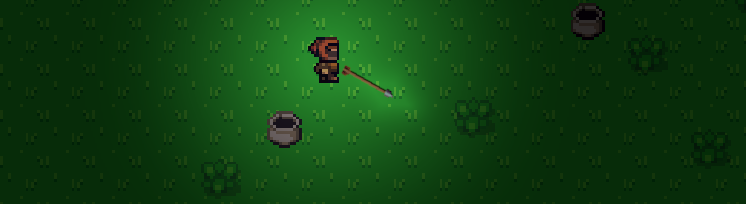
\includegraphics[width=1\textwidth]{images/ViseeFleche.png}
    \end{center}
    \captionof{figure}{Flèche suivant la direction de la souris}
Cette flèche est plus précisément celle qui indique la direction lorsque le bouton de la souris est relâché. Elle fournit ainsi une indication au joueur sur la possibilité de tirer et sur la direction dans laquelle la flèche sera tirée.
    \begin{center}
        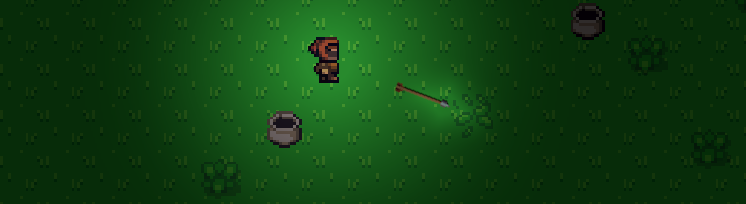
\includegraphics[width=1\textwidth]{images/FlecheDegats.png}
    \end{center}
    \captionof{figure}{Flèche détruisant un obstacle, en lui infligeant des dégats}
    La seule attaque qui ne fonctionne pas encore est la bombe de poison : la création de la zone à distance limitée fonctionne, mais celle-ci ne parvient pas encore à infliger des dégâts. De plus, l'animation de la bombe, allant du joueur jusqu'à la zone créée, n'a pas encore été implémentée.
    La zone de poison est limitée en distance grâce à un algorithme qui vérifie la distance entre le personnage et la position de la souris. De plus, une indication de l'emplacement de la zone de poison est affichée avant que le joueur déclenche l'attaque.
    \begin{center}
        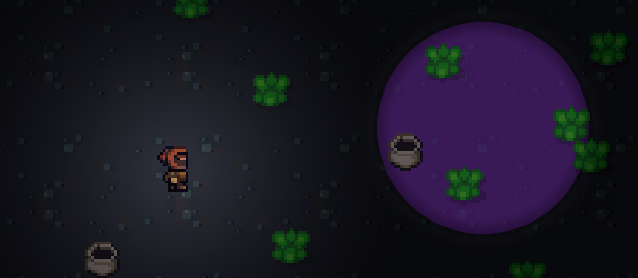
\includegraphics[width=1\textwidth]{images/PoisonZone.png}
    \end{center}
    \captionof{figure}{La zone de poison}
J'ai également veillé à ce que chaque élément ait une variable appelée "controlSpeed", qui permet de contrôler sa vitesse globale. Cela nous permettra ainsi d'implémenter facilement les pouvoirs liés au contrôle du temps, car pour accélérer ou ralentir le temps, il suffira de modifier cette variable.
}
    \subsubsection{Ressenti} {
Mon ressenti est plutôt positif, car je suis assez content de l'avancement du projet. \\ Il nous a également pris un certain temps afin de nous coordonner pour travailler efficacement en équipe, mais j'ai désormais le sentiment que nous pouvons aller plus vite qu'auparavant grâce à la dynamique d'équipe trouvée.
  }
\subsubsection{Axes d'Amélioration}{: L'apprentissage des bases d'Unity a pris une quantité considérable de temps, la maîtrise d'un nouveau logiciel n'étant pas une tâche simple. La recherche de documentation a également été difficile au début, étant donné que je ne connaissais ni les bases ni les termes spécifiques. Il est donc possible de gagner en rapidité sur ce point seul. \\ Nous pouvons également nous améliorer sur le travail en équipe, une meilleure communication et le travail simultané permettant de gagner un temps considérable et d'éviter des problèmes.
}
    \subsection{Marcus}
        \subsubsection{Travaux Réalisés} {
Pour le début de ce projet, j’ai obtenu des pistes audio de musique libre de droits correspondant à la direction artistique souhaitée pour notre jeu, ainsi que des effets sonores pour les événements. J’ai également récupéré des assets graphiques, tels que des sprites et des tilesets, sur des plateformes en ligne telles que Unity Asset Store, OpenGameArt et itch.io.

        Ensuite, je les ai modifiés afin de les rendre compatibles et utilisables dans notre projet. Ensuite, je les ai implémentés, ce qui impliquait la création d'une Tile Palette à partir de ces assets, l'assemblage des sprites pour créer les animations, et la modification de certains d’entre eux pour répondre à nos exigences techniques et artistiques.


        
        L'implémentation du fonctionnement des animations de base est une partie que j'ai appréciée, car j'ai trouvé le système d'animation de Unity très simple à prendre en main.
        En prenant l'exemple des animations du joueur, voici le graphe correspondant :
    \begin{center}
        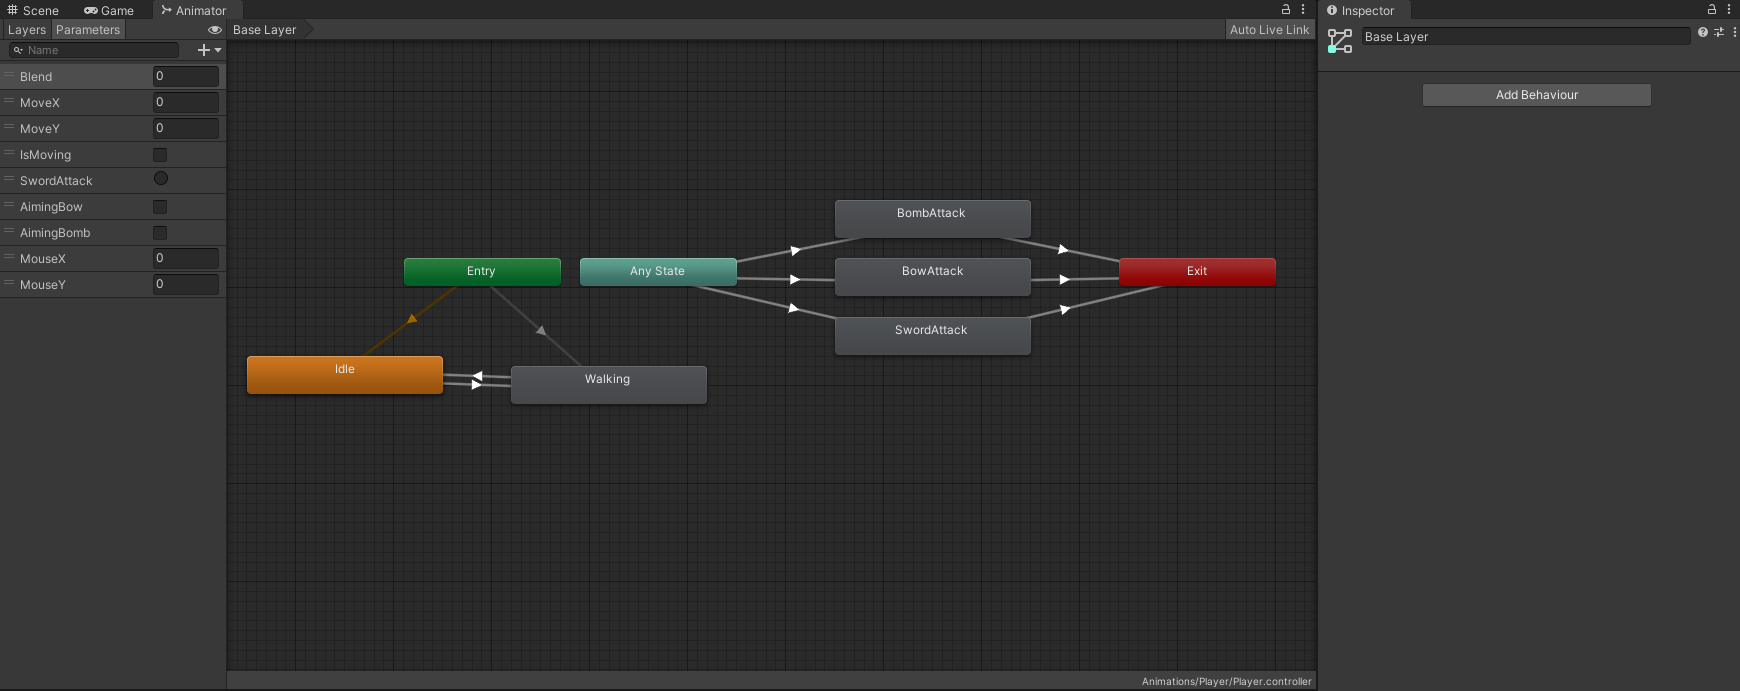
\includegraphics[width=1\textwidth]{images/Animator-Graph.png}
    \end{center}
    \captionof{figure}{Graphe de l'animateur du joueur}
    \begin{center}
        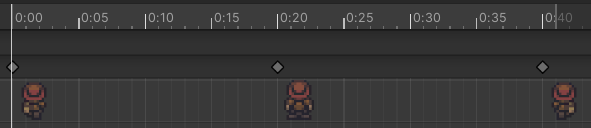
\includegraphics[width=1\textwidth]{images/Animationex.png}
    \end{center}
    \captionof{figure}{Exemple d'animation (vers le haut)}
Le fait de pouvoir déclencher une animation depuis n'importe quel état et à n'importe quel moment contribue énormément à simplifier les graphes. On obtient ainsi un mouvement et des animations entièrement fonctionnels à partir d'un graphe aussi simple. Chaque élément ici est un blend tree, un système très utile permettant de déclencher une animation en fonction de la valeur de différentes variables. C'est ainsi qu'on peut simplement déclencher l'animation correspondant à la direction indiquée par les flèches ou la souris (quand le joueur est en mode visée).
    \begin{center}
        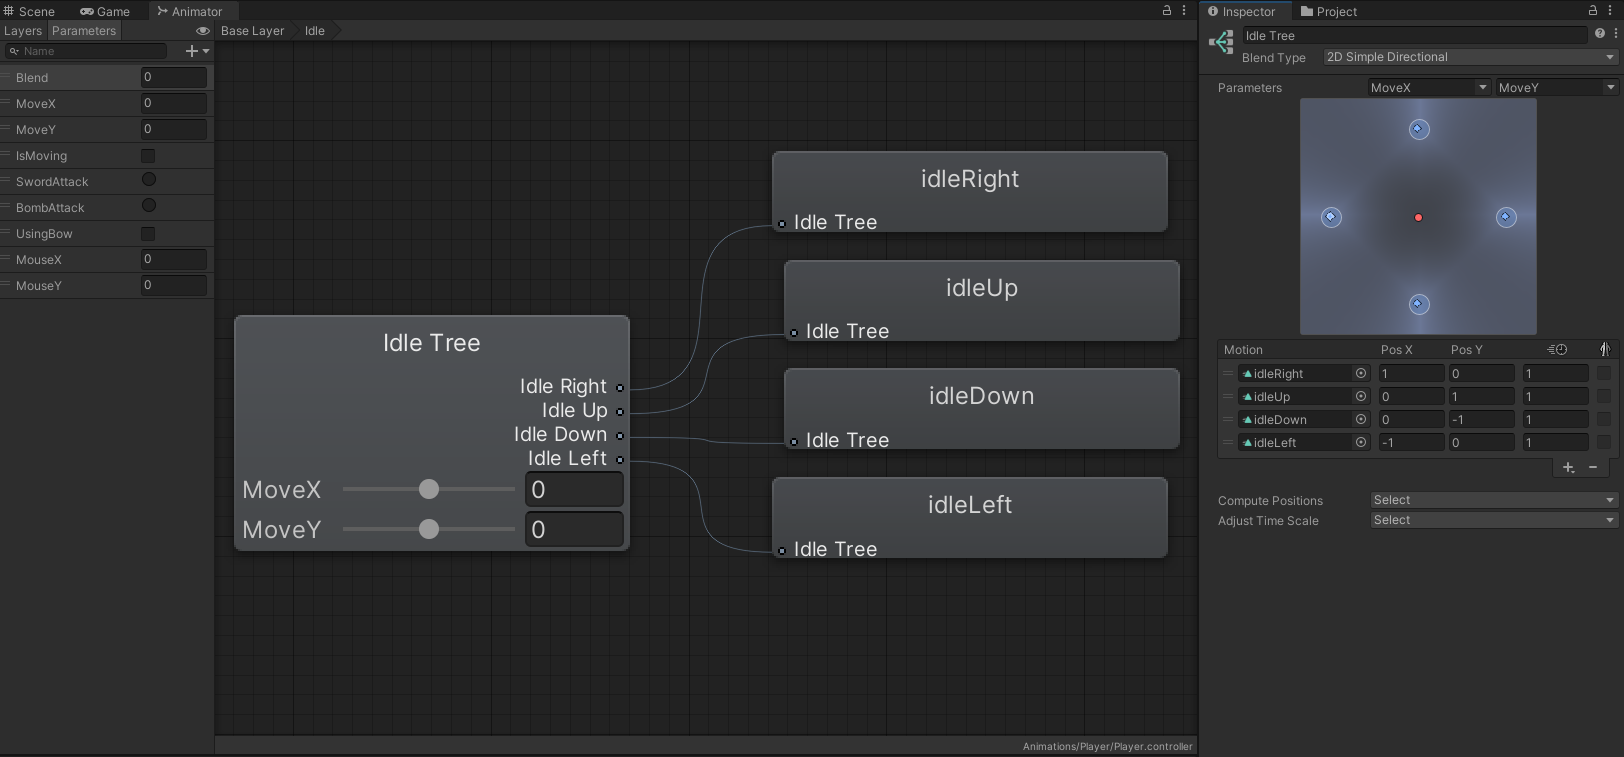
\includegraphics[width=1\textwidth]{images/BlendTree-Example.png}
    \end{center}
\captionof{figure}{BlendTree d'une animation du joueur}
Grâce à ces avancées, j'ai déjà pu essayer mes assets dans une scène et tester leur qualité, leur compatibilité entre eux ainsi que les effets de lumière propres à notre jeu. Ici, je teste les animations ainsi que la lumière dynamique des torches, des lampes et d'un interrupteur.
     \begin{center}
        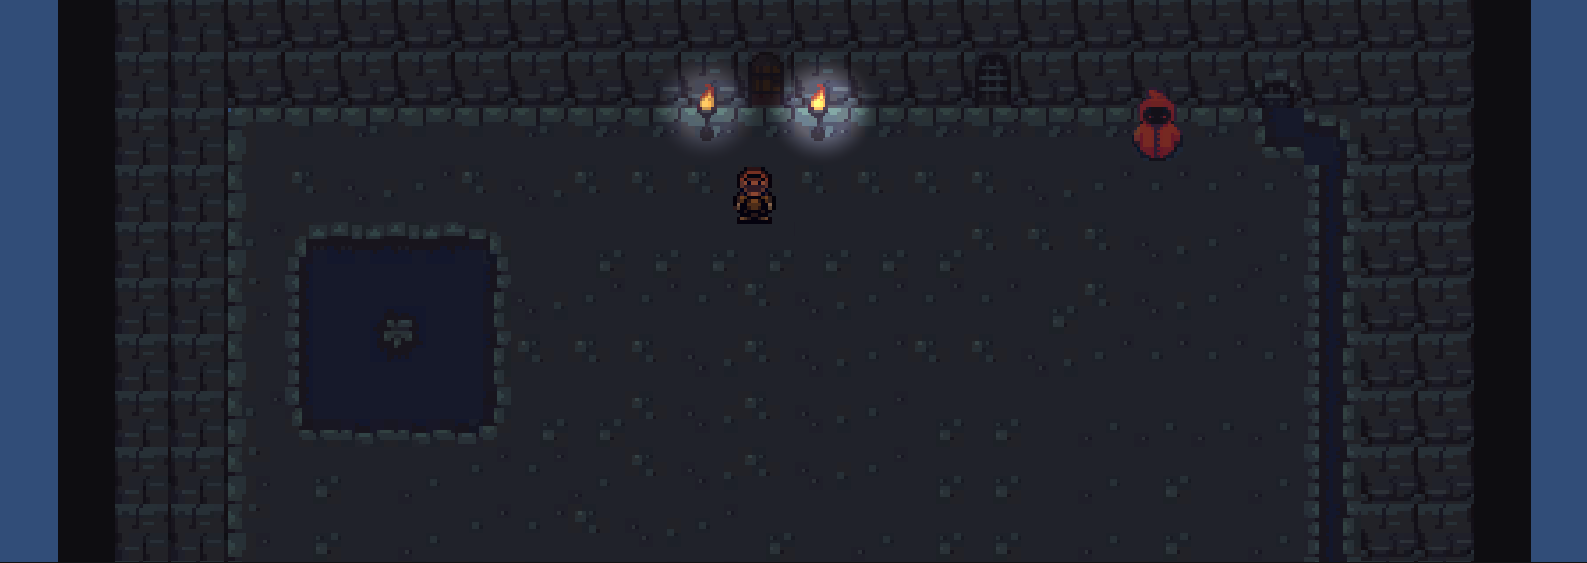
\includegraphics[width=1\textwidth]{images/ImageCave}  
        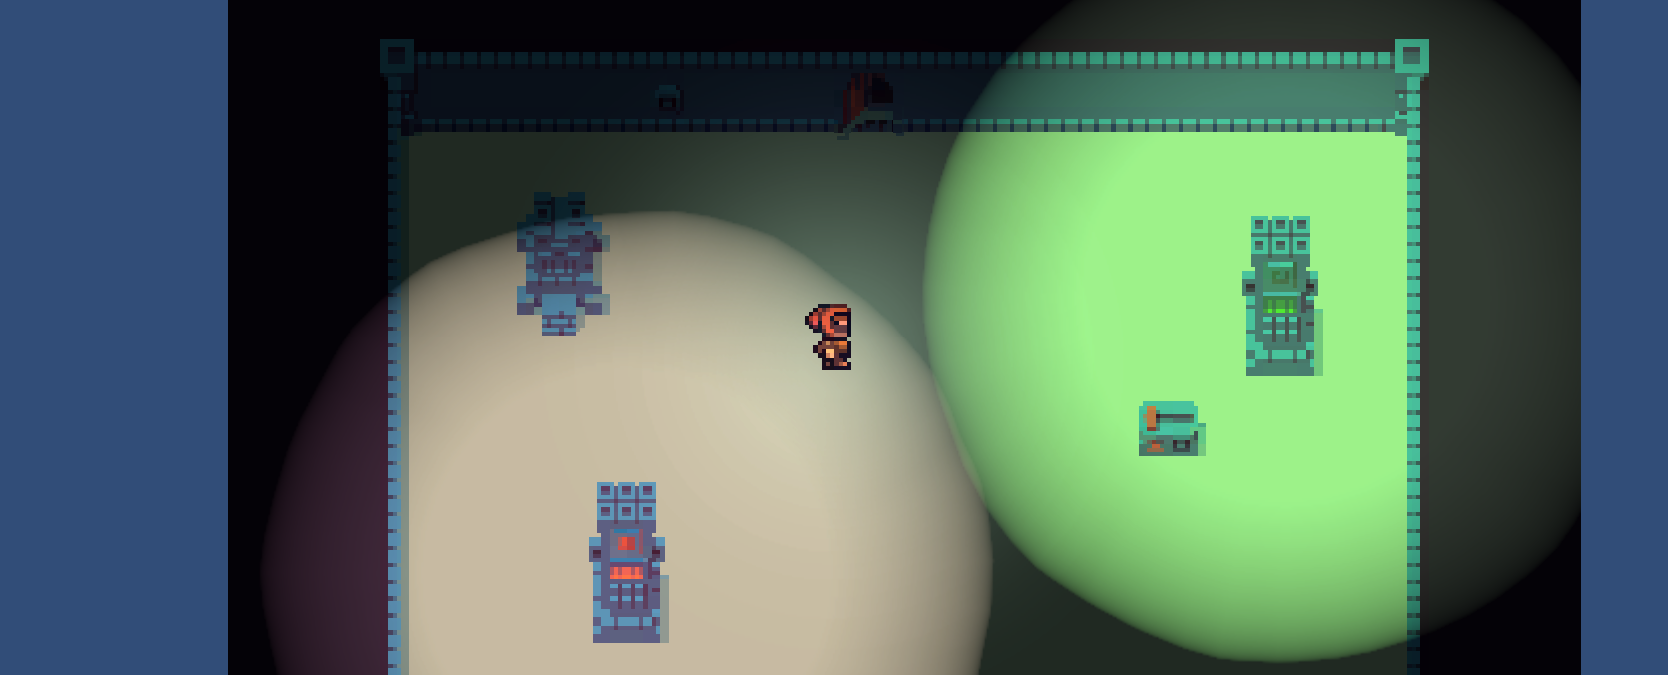
\includegraphics[width=1\textwidth]{images/imageCave2.png} 
    \end{center}
\captionof{figure}{Images d'un dongeon de Test} 
}
        \subsubsection{Ressenti Personnel}
La prise en main de Unity n'a pas été rapide. Certaines implémentations et améliorations ont dû être refaites plus d'une fois en raison d'un manque de compréhension de GitHub et de Unity. Cependant, l'utilisation de nouveaux outils qui mêlent l'art et la programmation a été très rafraîchissante et m'a motivé à m'investir encore plus dans ce projet.
        \subsubsection{Axes d'Amélioration}
La prise en main de Unity ayant pris une part conséquente du travail des premières semaines, je devrais améliorer ma maîtrise de Unity ainsi que des outils de montage photo pour accélérer l'implémentation des prochaines tâches. De plus, je devrais travailler sur la création de plus de sprites originaux afin d'augmenter la variété du bestiaire et du décor, sans oublier l'implémentation des effets audio tels que les musiques et l'audio dynamique du jeu. . 
    \subsection{Louis}
        \subsubsection{Travaux Réalisés}
            {Au cours de ces dernières semaines, j'ai pu collaborer sur ce projet de projectiles avec Quentin, corriger les mouvements des objets dans le jeu, et j'ai aussi commencé à m'occuper des ennemis.
            
            En ce qui concerne les déplacements du personnage et ceux de nos projectiles, le problème était qu'ils n'étaient pas du tout fluides mais plutôt saccadés, avec une vitesse qui n'était pas constante ou du moins ne le paraissait pas. J'ai donc modifié la méthode avec laquelle nous déplacions les objets dans le monde de Zelion en utilisant quelques recommandations trouvées sur internet.
            
            Enfin, pour les ennemis, j'ai implémenté le tir de flèches ou d'autres projectiles ainsi que l'attaque rapprochée des ennemis (nous avons encore besoin des sprites des ennemis et de leurs animations). Malheureusement, je n'ai pas encore réussi à implémenter leur déplacements.}
        \subsubsection{Ressenti Personnel}
            {Personnellement, cela m'a un peu frustré car j'ai tenté sans relâche d'implémenter le déplacement des ennemis, mais cela n'a abouti à rien. J'y ai passé beaucoup trop de temps à essayer de déterminer ce qui ne fonctionnait pas. J'ai même utilisé d'autres projets Unity ainsi que des versions différentes de Unity, mais je n'ai pas réussi à faire fonctionner les déplacements sur Zelion (et seulement un de mes tests a réussi, mais je n'ai pas compris pourquoi). Cela m'a vraiment frustré, surtout compte tenu du temps que j'y ai consacré sans résultat.
            
            Mais bon, cela n'est pas trop grave, étant donné que cela m'a vraiment fait plaisir de travailler avec les autres et de nous aider mutuellement.
            
            J'ai pu ainsi me réhabituer à Unity (j'avais déjà réalisé un petit projet personnel avec un ami au lycée) et j'ai appris à mieux maîtriser Unity en élargissant le nombre d'outils du moteur disponibles pour moi.}
        \subsubsection{Axe d'Amélioration}
            {Je pense que j'ai passé trop de temps bloqué sur un seul problème. J'aurais dû me concentrer sur d'autres tâches afin que, au moment de revenir sur ce problème, j'aurais peut-être eu d'autres idées. Je le sais bien, étant donné que cela m'est déjà arrivé plusieurs fois, mais j'ai tendance à penser que je peux facilement trouver la solution.
    Je pense aussi qu'on aurait dû commencer à travailler ensemble plus tôt, c'est-à-dire se retrouver à un endroit pour travailler sur le projet.}
    \subsection{Adrien}
        \subsubsection{Travaux Réalisés}
    {Lors de ces premiers mois de travail, j'ai eu l'occasion de participer au développement des mouvements de base (déplacement en deux dimensions), ainsi qu'aux premières versions de l'esquive qui seront par la suite améliorées au fur et à mesure des idées de notre équipe. En parallèle, j'ai aussi codé les différentes barres de ressources (vie, mana, endurance) et ai relié certaines actions à ces barres. Par exemple, effectuer une esquive vous fera perdre de l'endurance, qui se régénérera avec le temps.}
\subsubsection{Ressenti Personnel}
    {Participer au développement du début de Zelion a été une expérience enrichissante pour moi. J'ai vraiment apprécié cette opportunité, car cela m'a permis de m'inspirer des jeux auxquels j'avais déjà joué afin de mieux comprendre comment les différentes mécaniques pouvaient être implémentées. En m'immergeant dans ce processus de création, j'ai pu saisir de plus en plus les mécanismes sous-jacents des jeux vidéo et apprécier davantage les jeux vidéo en général. Chaque ligne de code que j'ai écrite m'a permis de mieux appréhender la manière dont les autres jeux ont été conçus, tout en stimulant ma créativité pour ce projet. Cette expérience m'a permis de réaliser la complexité et la beauté de la programmation dans le domaine du jeu vidéo.
    \\ Bien sûr, il y a eu aussi quelques problèmes durant cette première partie de programmation. En effet, la grande motivation que j'avais en début d'année s'est vite essoufflée avant de faire son grand retour il y a quelques semaines grâce aux propositions de travail groupé à l'EPITA de la part de notre chef de projet...}
\subsubsection{Axes d'Améliorations}
    {Afin de m'améliorer, je pense que je devrais renforcer ma maîtrise de GitHub, ce qui me permettra d'être plus efficace lors du partage de fichiers avec mes collègues. Bien sûr, je devrais aussi continuer sur cette lancée de motivation qui nous a tous poussés en cette fin de bimestre, afin de ne pas prendre de retard sur le projet.}
\section{Objectifs pour la prochaine soutenance} {
    Pour la prochaine soutenance, nous avons pour objectif de finaliser entièrement notre jeu.
    
    Voici donc le travail qu'il nous reste à fournir pour chaque tâche :
    \subsection{Noyau du gameplay} {
Nous devons achever l'implémentation des attaques, en particulier celle de la bombe de poison. De plus, nous devrons également coder les capacités liées au contrôle du temps, c'est à dire le ralentissement du temps et le retour en arrière.
}
    \subsection{Interface Utilisateur} {
    Les barres de vie, d'endurance et de mana sont désormais réalisées, tout comme les dialogues. Il nous reste désormais à créer tous les menus, y compris l'écran d'accueil et le menu de pause.
    }

    \subsection{IA - Ennemis} {    
    Pour la prochaine soutenance, il faudra que nous implémentions les déplacements des ennemis. De plus, nous devrons aussi ajouter les boss et leur donner des capacités spécifiques, en plus d'attribuer des caractéristiques à chaque type d'ennemi.

    Il nous manque aussi les sprites et les animations.
    }

    \subsection{Graphismes} {
    Les sprites finaux ont été trouvés et en partie animés, et les effets de lumière sont fonctionnels.
    
    Ce qu'il nous reste à accomplir est donc l'animation des ennemis, l'animation certains éléments du décor, et à peaufiner les animations existantes.
    }
    \subsection{Sound Design} {
Les bruitages et les musiques doivent encore être intégrés. Cependant, la plupart des fichiers que nous allons utiliser ont déjà été préparés.
    }
    \subsection{Écriture}{
    L'histoire est conçue, il ne reste qu'à implémenter les dialogues.
    }
    \subsection{Level Design} {
    Nous avons des idées de niveau et de mécaniques de prêtes, mais le jeu n'est pas encore assez avancé pour les implémenter. 
    }
    \subsection{Multijoueur} {
    Pas encore commencé.
    }
}
\section{Conclusion} {
    
Pour conclure, ces premiers mois de travail sur le projet ont été une expérience enrichissante pour nous tous.

En effet, nous avons appris l'importance du travail d'équipe pour progresser efficacement, et nous avons désormais les bases et la confiance nécessaires pour nous permettre de mener ce projet à terme.

Nous sommes ainsi motivés à terminer Zelion d'ici la prochaine soutenance.
}

\section{Annexes}
    \subsection{Site Web}
        \begin{center}
        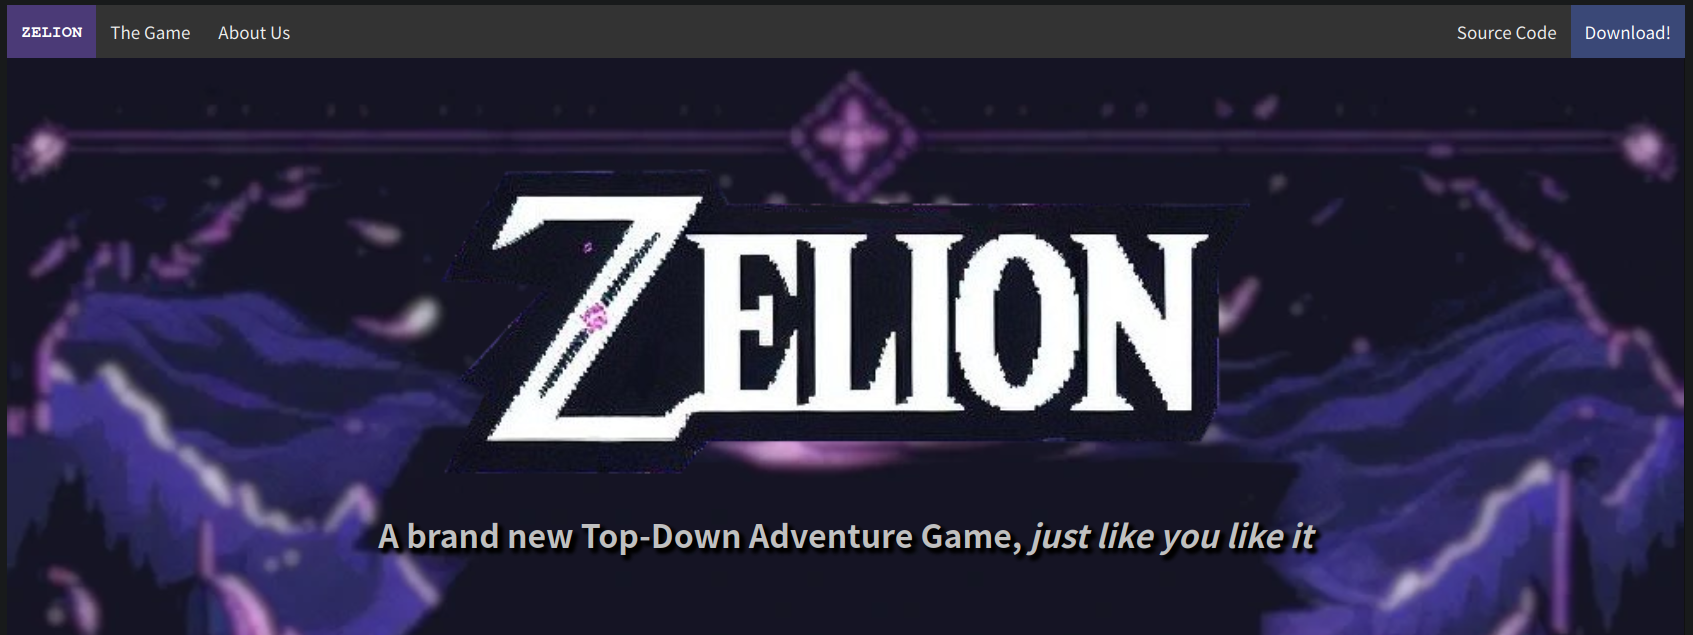
\includegraphics[width=1\textwidth]{images/WebsiteScreenshot1.png}
    \end{center}
    \captionof{figure}{Accueil du site web de Zelion} 
    \subsection{Asset Graphique}
    \begin{center}
      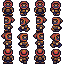
\includegraphics[width=0.4\textwidth]{images/Rogue.png}
    \end{center}
\captionof{figure}{Sprites du personnage principal, avec ses animations}
    \begin{center}
          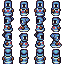
\includegraphics[width=0.4\textwidth]{images/Mage.png}
             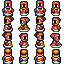
\includegraphics[width=0.4\textwidth]{images/MageRed.png}
    \end{center}
\captionof{figure}{Exemple de deux ennemis}

\begin{center}
      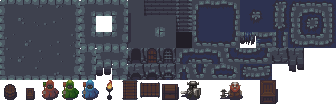
\includegraphics[width=16cm]{images/dungeon_tiles_compact_and_varied.png}
    \end{center}
\captionof{figure}{Tileset du dongeon}

\newpage
\renewcommand{\listfigurename}{Liste des Figures}
\renewcommand{\listtablename}{Liste des Tables}

\listoftables
\listoffigures

\end{document}

